\documentclass[../manuale-utente.tex]{subfiles}

\begin{document}

\subsection{Preparazione del predittore}
\label{subs:preparazione-del-predittore}
Prima di tutto si dovrà avere a disposizione un file JSON ottenuto dall'addestramento.

\begin{figure}[h!]
  \begin{center}
    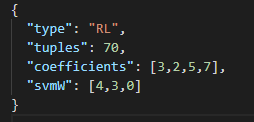
\includegraphics[width=8cm]{esempioFileJson.png}\\
    \caption{Esempio di file JSON}%
    \label{fig:esempio-filejson}
  \end{center}
\end{figure}

\subsection{Configurazione del plug-in}
\label{subs:configurazione-plug-in}
Una volta avviato Grafana sarà neccessario andare alla pagina di configurazione e una volta selezionata la voce "Plugins" si
dovrà cliccare la barra di ricerca e scrivere "CoffeeCode".

\begin{figure}[h!]
  \begin{center}
    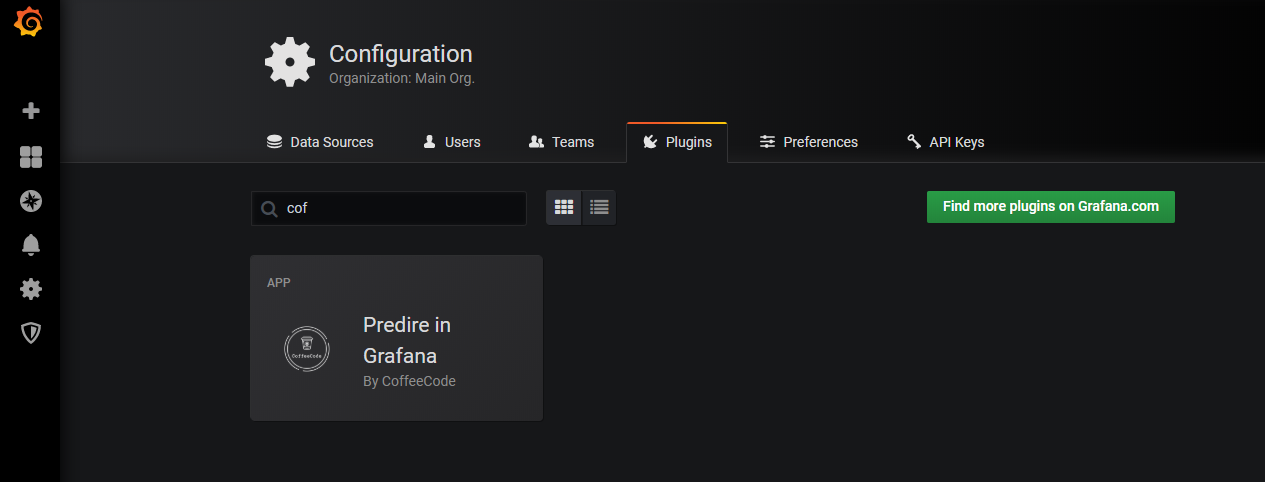
\includegraphics[width=17cm]{configurazionePlugIn-pt1.png}\\
    \caption{Pagina di configurazione di Grafana}%
    \label{fig:pagina-di-configurazione}
  \end{center}
\end{figure}

Trovata l'applicazione bisognerà cliccarci sopra e premere il tasto "Enable" per abilitare il plug-in.

\begin{figure}[h!]
  \begin{center}
    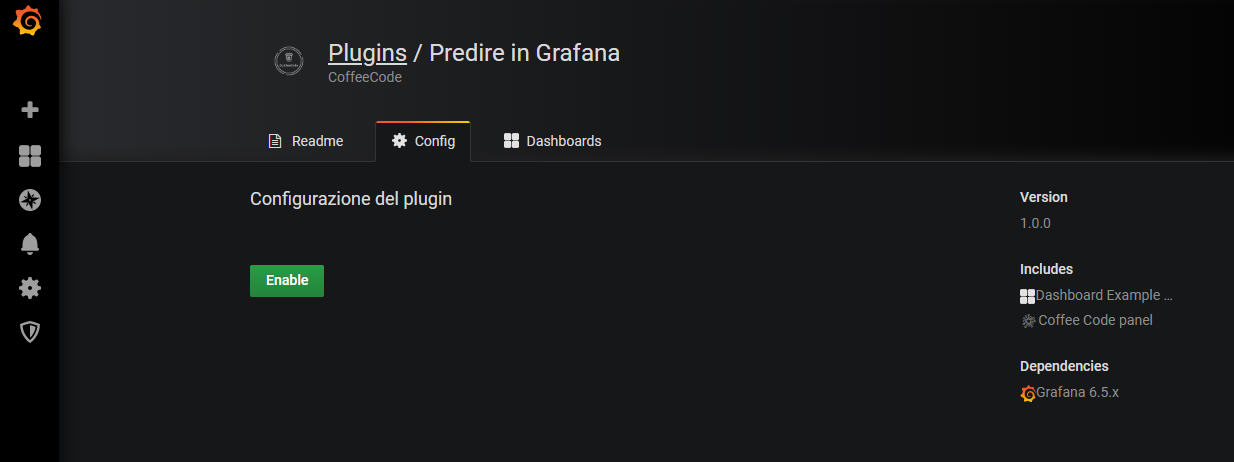
\includegraphics[width=17cm]{configurazionePlugIn-pt2.png}\\
    \caption{Tasto "Enable"}%
    \label{fig:tasto-enable}
  \end{center}
\end{figure}

\newpage
\subsection{Creazione di un Pannello}
\label{subs:creazione-di-un-pannello}
Per aggiungere il pannello si dovrà andare alla Dashboard e cliccare in alto a destra su "Add Panel".

\begin{figure}[h!]
  \begin{center}
    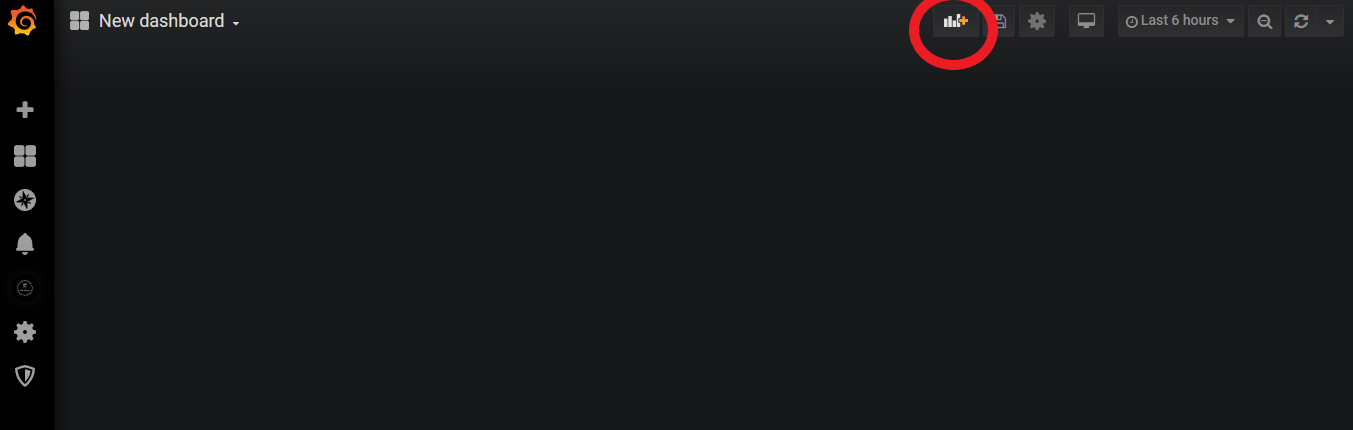
\includegraphics[width=17cm]{aggiungiPannelloPlugIn-pt1.png}\\
    \caption{Cliccare dove indicato col cerchio rosso}%
    \label{fig:aggiungi-pannello}
  \end{center}
\end{figure}

Aggiunto il pannello ci verra chiesto di scegliere il tipo di visualizzazione e si dovrà cliccare su "Choose Visualization".

\begin{figure}[h!]
  \begin{center}
    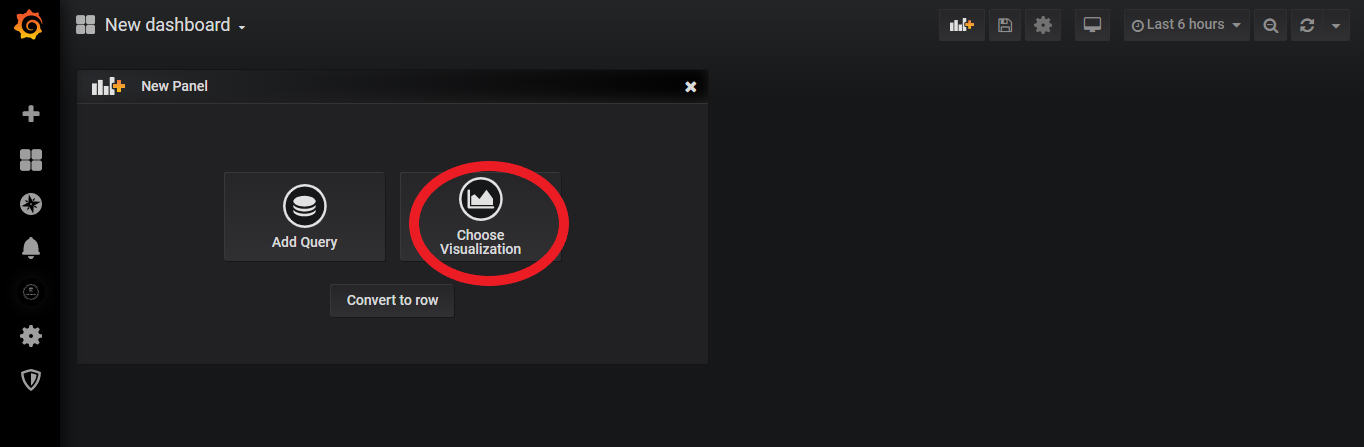
\includegraphics[width=17cm]{aggiungiPannelloPlugIn-pt2.png}\\
    \caption{Cliccare dove indicato col cerchio rosso}%
    \label{fig:scegliere-la-visualizzazione}
  \end{center}
\end{figure}

\newpage
\subsection{Configurazione del pannello}

Si dovrà trovare il "Coffee Code Panel" e cliccarci sopra così da far comparire il pulsante "scegli file" per caricare il predittore in formato JSON.

\begin{figure}[h!]
    \begin{center}
      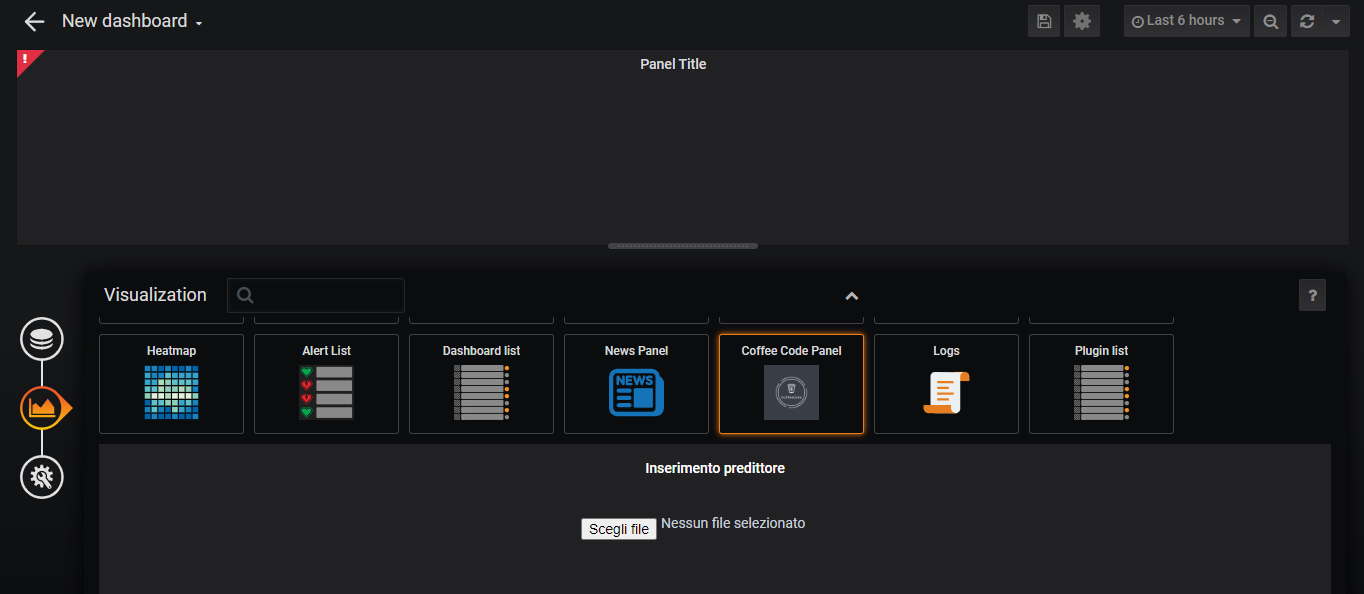
\includegraphics[width=17cm]{aggiungiPannelloPlugIn-pt3.png}\\
      \caption{Premere su "scegli file"}%
      \label{fig:scelta-del-file}
    \end{center}
  \end{figure}

Una volta caricato il file bisognerà impostare almeno 2 query dalle quali verranno presi i dati per calcolare la predizione.

\begin{figure}[h!]
    \begin{center}
      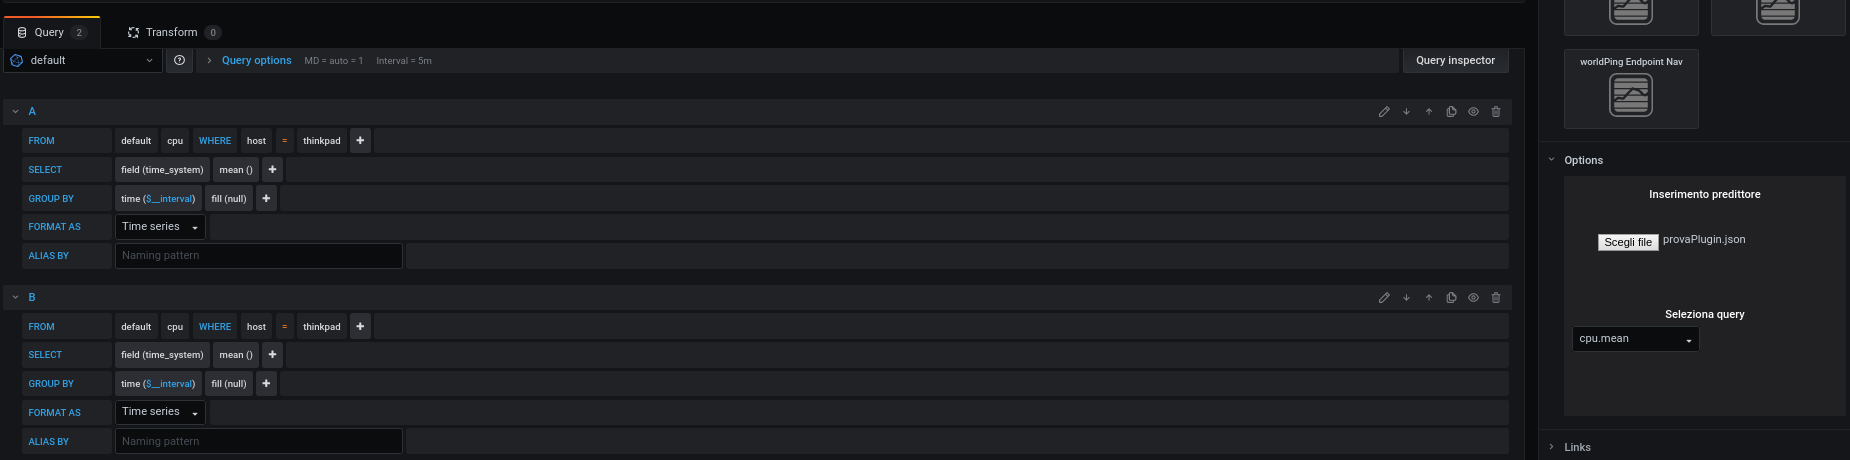
\includegraphics[width=17cm]{querySample.png}\\
      \caption{Selezionare le query}%
      \label{fig:selezionare-le-query}
    \end{center}
  \end{figure}
  \newpage
Per concludere la configurazione si dovrà aggiornare la pagina e si visualizzerà il grafico con la predizione.

\begin{figure}[h!]
    \begin{center}
      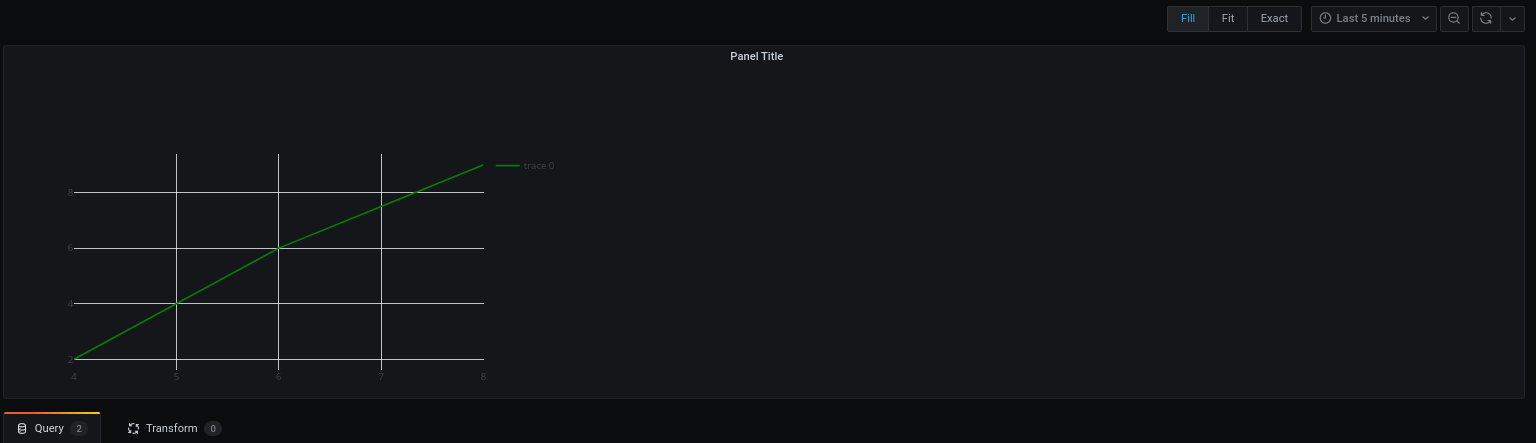
\includegraphics[width=17cm]{graficoSample.png}\\
      \caption{Esempio di grafico che verrà visualizzato}%
      \label{fig:esempio-grafico}
    \end{center}
  \end{figure}

\end{document}
